\section{Corba\-Consumer\-Base Class Reference}
\label{classCorbaConsumerBase}\index{CorbaConsumerBase@{CorbaConsumerBase}}
Inheritance diagram for Corba\-Consumer\-Base::\begin{figure}[H]
\begin{center}
\leavevmode
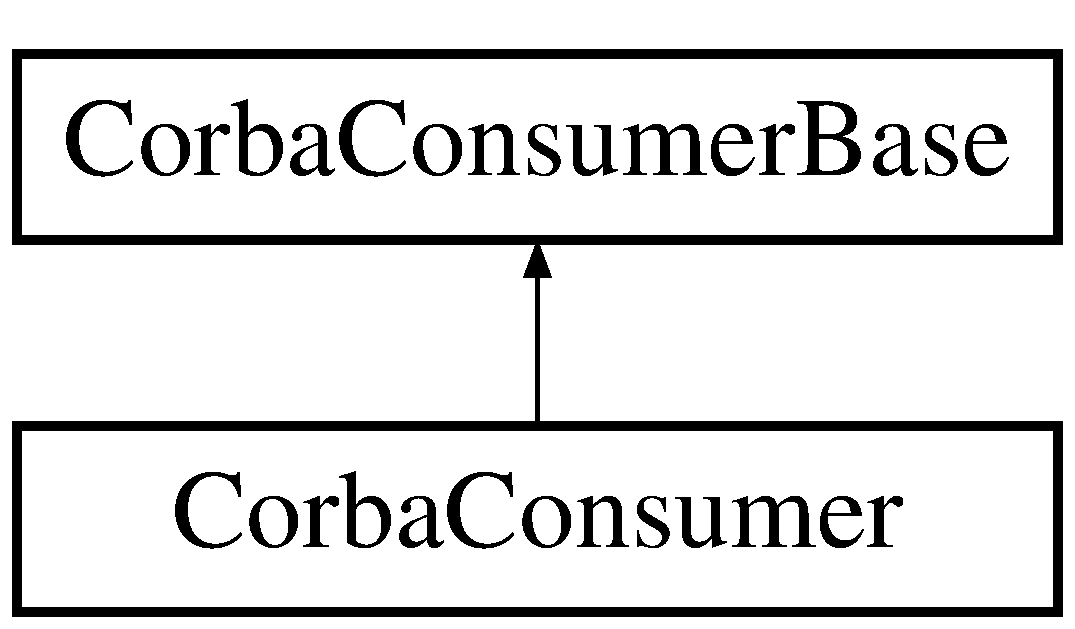
\includegraphics[height=2cm]{classCorbaConsumerBase}
\end{center}
\end{figure}
\subsection*{Public Member Functions}
\begin{CompactItemize}
\item 
{\bf \_\-\_\-init\_\-\_\-} (consumer=None)
\begin{CompactList}\small\item\em Consructor. \item\end{CompactList}\item 
{\bf equal} (consumer)
\item 
{\bf \_\-\_\-del\_\-\_\-} ()
\begin{CompactList}\small\item\em Destructor. \item\end{CompactList}\item 
{\bf set\-Object} (obj)
\begin{CompactList}\small\item\em Set CORBA Object. \item\end{CompactList}\item 
{\bf get\-Object} ()
\begin{CompactList}\small\item\em Set CORBA Object. \item\end{CompactList}\item 
{\bf release\-Object} ()
\end{CompactItemize}


\subsection{Member Function Documentation}
\index{CorbaConsumerBase@{Corba\-Consumer\-Base}!__del__@{\_\-\_\-del\_\-\_\-}}
\index{__del__@{\_\-\_\-del\_\-\_\-}!CorbaConsumerBase@{Corba\-Consumer\-Base}}
\subsubsection{\setlength{\rightskip}{0pt plus 5cm}Corba\-Consumer\-Base::\_\-\_\-del\_\-\_\- ()}\label{classCorbaConsumerBase_CorbaConsumerBasea2}


Destructor. 



Reimplemented in {\bf Corba\-Consumer} {\rm (p.\,\pageref{classCorbaConsumer_CorbaConsumera2})}.\index{CorbaConsumerBase@{Corba\-Consumer\-Base}!__init__@{\_\-\_\-init\_\-\_\-}}
\index{__init__@{\_\-\_\-init\_\-\_\-}!CorbaConsumerBase@{Corba\-Consumer\-Base}}
\subsubsection{\setlength{\rightskip}{0pt plus 5cm}Corba\-Consumer\-Base::\_\-\_\-init\_\-\_\- (consumer = {\tt None})}\label{classCorbaConsumerBase_CorbaConsumerBasea0}


Consructor. 

\index{CorbaConsumerBase@{Corba\-Consumer\-Base}!equal@{equal}}
\index{equal@{equal}!CorbaConsumerBase@{Corba\-Consumer\-Base}}
\subsubsection{\setlength{\rightskip}{0pt plus 5cm}Corba\-Consumer\-Base::equal (consumer)}\label{classCorbaConsumerBase_CorbaConsumerBasea1}




Reimplemented in {\bf Corba\-Consumer} {\rm (p.\,\pageref{classCorbaConsumer_CorbaConsumera1})}.\index{CorbaConsumerBase@{Corba\-Consumer\-Base}!getObject@{getObject}}
\index{getObject@{getObject}!CorbaConsumerBase@{Corba\-Consumer\-Base}}
\subsubsection{\setlength{\rightskip}{0pt plus 5cm}Corba\-Consumer\-Base::get\-Object ()}\label{classCorbaConsumerBase_CorbaConsumerBasea4}


Set CORBA Object. 

return The CORBA Object reference that given by {\bf set\-Object(obj)}{\rm (p.\,\pageref{classCorbaConsumerBase_CorbaConsumerBasea3})} \begin{Desc}
\item[Returns:]obj Object reference of CORBA object\end{Desc}
\index{CorbaConsumerBase@{Corba\-Consumer\-Base}!releaseObject@{releaseObject}}
\index{releaseObject@{releaseObject}!CorbaConsumerBase@{Corba\-Consumer\-Base}}
\subsubsection{\setlength{\rightskip}{0pt plus 5cm}Corba\-Consumer\-Base::release\-Object ()}\label{classCorbaConsumerBase_CorbaConsumerBasea5}




Reimplemented in {\bf Corba\-Consumer} {\rm (p.\,\pageref{classCorbaConsumer_CorbaConsumera5})}.\index{CorbaConsumerBase@{Corba\-Consumer\-Base}!setObject@{setObject}}
\index{setObject@{setObject}!CorbaConsumerBase@{Corba\-Consumer\-Base}}
\subsubsection{\setlength{\rightskip}{0pt plus 5cm}Corba\-Consumer\-Base::set\-Object (obj)}\label{classCorbaConsumerBase_CorbaConsumerBasea3}


Set CORBA Object. 

The given CORBA Object is held. \begin{Desc}
\item[Parameters:]
\begin{description}
\item[{\em obj}]Object reference of CORBA object \end{description}
\end{Desc}
\begin{Desc}
\item[Returns:]If obj is nil reference, it returns false.\end{Desc}


Reimplemented in {\bf Corba\-Consumer} {\rm (p.\,\pageref{classCorbaConsumer_CorbaConsumera3})}.

The documentation for this class was generated from the following file:\begin{CompactItemize}
\item 
{\bf Corba\-Consumer.py}\end{CompactItemize}
